\documentclass[conference]{IEEEtran}
\IEEEoverridecommandlockouts
% The preceding line is only needed to identify funding in the first footnote. If that is unneeded, please comment it out.
\usepackage{cite}
\usepackage{amsmath,amssymb,amsfonts}
\usepackage{algorithmic}
\usepackage{graphicx}
\usepackage{textcomp}
\usepackage{xcolor}
\usepackage{algorithm2e}
\def\BibTeX{{\rm B\kern-.05em{\sc i\kern-.025em b}\kern-.08em
    T\kern-.1667em\lower.7ex\hbox{E}\kern-.125emX}}
\begin{document}

\title{Smart Traffic Lights with RSUs\\
	{\footnotesize \textsuperscript \  }
	\thanks{}
}

\author{\IEEEauthorblockN{ Adnan CIGTEKIN}
	\IEEEauthorblockA{\textit{Department of computer science} \\
		\textit{Yeditepe University}\\
		Istanbul, Turkey \\
	adnan.cigtekin@std.yeditepe.edu.tr}
	\and
	\IEEEauthorblockN{ Berkay KOCAK}
	\IEEEauthorblockA{\textit{Department of computer science} \\
		\textit{Yeditepe University}\\
		Istanbul, Turkey \\
	berkay.kocak@std.yeditepe.edu.tr}
	\and
	\IEEEauthorblockN{ Gorkem KAR}
	\IEEEauthorblockA{\textit{Department of computer science} \\
		\textit{Yeditepe University}\\
		Istanbul, Turkey \\
	gkar@cse.yeditepe.edu.tr}
	
}

\maketitle

\begin{abstract}
	Current traffic lights approach is based on predefined cycles or manual control. This  primitive approach for handling the lights creates an environment that cannot be scalable  for its current traffic situation. According to our observations current system is prone to be inefficient. Because, in current system the duration of red and green lights are static. However, the car amount in the traffic varies through the day. This causes unnecessary waiting time for the vehicles in the traffic. Even with the light duration which have been calculated beforehand according to congestion of the traffic through the day, we still can't overcome the possibility of exceptions. For example, when someone important or famous uses that road unexpectedly, the traffic at the lights will increase and people will start to wait longer at the lights. This might cause problems even for economics of that country.\cite{a1} So, this problem must be solved. To solve this issue we developed a new approach.
\end{abstract}
\iffalse Assign links to abbreviations with our approach.\fi
\begin{IEEEkeywords}
	RSU(Road size unit)
\end{IEEEkeywords}

\section{Introduction}
Traffic congestion is main problem of modern transportation.There is many sides of this problem such as, driver faults, insufficient road designs,  inadequate control systems etc.Among all these problems our subject is traffic lights and their reflection on congestion.In our researches, different timings on traffic light creates discrete congestion.With this observed difference, we can build a new structure to provide a new approach on traffic congestion.
\\
In this paper we will compare predefined manual traffic lights with aligned traffic lights with our proposed solution. 
Our approach is about calculating cars on the road and optimizing the lights on behalf the calculated data. For processing the data , we can use weight based priority algorithms with road superiority restrictions.As for the real life implementation, we can use road side units(RSU) to calculate car number on a road via their connections to RSU and after the data collected we can distribute it to algorithm to decide traffic lights cycles. With this system, we will be able to change the duration of red and green lights according to current congestion in the road. So, the light duration of red and green lights will change dynamically through the day. With this approach we can ease the congestion problem created by traffic lights also we can arrange the road flow for the high priority vehicles like ambulance and we can increase develop the economy of that country in the long-run. 


\section{BACKGROUND, RELATED WORKS AND OUR CONTRIBUTIONS}

\subsection{Current Approaches}

For normalizing the flow of traffic there are already some methods. One of the method is putting surveillance cameras on top of the traffic lights. With these cameras there are two techniques to regulate the traffic.
\begin{enumerate}
	\item Assigning a person to watch the camera outputs and then detect in which hours the traffic is congested or not.
	\item Using image recognition and machine learning techniques to overcome the need for humans. The AI behind this process does the same thing as humans assigned to do this job.
\end{enumerate}

\subsection{Problems of Current Approaches}
\begin{enumerate}
	\item Assigning a human :
	      \begin{itemize}
	      	\item Assigning a worker to implement traffic lights timer calculations is inefficient and it is bound to affiliate with human error.
	      	\item Continuous loss of money for wages of human workers.
	      \end{itemize}
	\item Using recognition and machine learning :
	      \begin{itemize}
	      	\item Hard to get accurate data sets to train AI with machine learning techniques. 
	      	\item It needs high level computation power for every new training sets.
	      \end{itemize}
	      \iffalse \textbf{we may back this accusation with individual data sets} \fi
\end{enumerate}
In our project, we are trying to solve these problems and develop a complete structure with intelligent design.


\section{Design}
Our design consists of 3 parts, which are;
\begin{enumerate}
    \item Calculation and Decision:
    This part is handled via Artificial Intelligence on a central server which has been explained in detail at next section.Moreover, this part is the most crucial component of the proposed method because includes decision and calculations.
    \\
    \item Core Network: 
    In this component, there is no any specific development done in our proposed method scope.It uses traditional network methods to connect RSU network to Central Server.
    \\
     \item Local RSU Network: 
     Local RSU network component gathers two type of information.Car amount and connected cars.
     With these data we can feed our AI to make decisions on congested areas.Moreover, we can think these local RSU networks as a intranet for local vehicle-to-vehicle and vehicle-to-RSU communications.Therefore, local RSU networks connected distinctly to the core network.
This design can be observed at (figure 1).

\end{enumerate}




 \begin{figure}[h!]
     \centering
     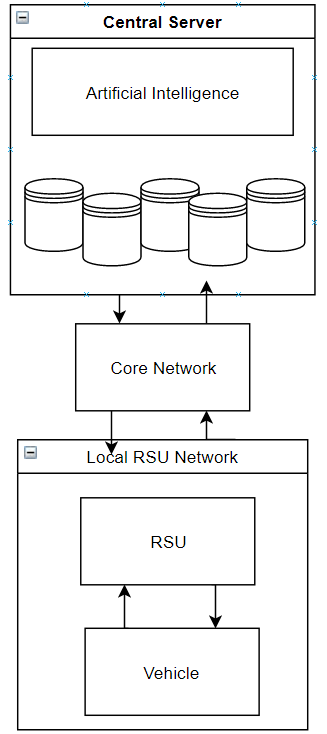
\includegraphics[width=6cm]{arc.PNG}
     
     \caption{General Design.}
     \label{fig:my_label}
     
 \end{figure} 
In the end as a summarization, cars are connected to the RSU and these RSU's counts cars then posts this information to core network at last AI collects information and begins to process.Then posts back these results to corresponding RSU's. 

\section{Artificial Intelligence And Calculations}
Artificial Intelligence is needed due to different and changing road situations.System must respond these situations with different manners.Thus, we have developed our own field specific AI to handle difference environments.
\\

\subsection{Rsu Assumptions}
    There are several assumptions on AI to implement the prototype of our project and to create realistic test cases on simulations.
    \begin{itemize}
	      	\item RSU location is calculated separately to determine the minimum required distance.However in our AI, it has been assumed RSU is always in the required range.
	      	\\
	      	\item Test environment of the project is a simulation of perfect traffic congestion.Which means all the drivers obey traffic rules and has constant acceleration levels.This assumption has been done to ease the test cases.Although our project scope is determined with prototype.Thus implementing these features would be out of our scope. 
	\end{itemize}
\subsection{Rsu Calculations}
 There is several calculations done in our system due to determine the different conditions on environment.
    \begin{itemize}
	      	\item One of the calculations is about minimum required distance between RSU to traffic light.This distance is needed because RSU car counting depends on cycles.Cycle length also depends on different calculations which explained at next step.However in this step , we are calculating minimum required distance as ;
	      	\begin{equation}
            \frac{Road Limit (km/hour) }{\frac{1}{hour}}
            \end{equation} 
	      	\item Next calculation is about observation time which we referred as car counting cycle length at previous step.This calculation is critical because car numbers are the main variable of our structure and counting cycles involves directly to these counts.Calculation formula for the cycle length; 
	      	\begin{equation}\frac {Min. Req. Dist. from RSU-to-Traffic Light ( km )} { Road Limit ( km/h )} \end{equation} 

	\end{itemize}
\subsection{AI Template}
In this sections a simple pseudo code will be presented.Sub statements will not be shown in detail for the sake of simplicity.
\begin{algorithm}
\SetAlgoLined

Connect to RSU\;
Get road type\;
Get car count\;
Initialize calculations\;\

\While{car count cycle != end}{
 
Get road intersection information\;
MPR = Get most priority road \;
CCR = Get most car count road \;

  \uIf{MPR.priorityRate == CCR.priorityRate}{
    Check for sub statements\;
    Then calculate light times\;
   }\uElseIf{MPR.carAmount \textless  CCR.carAmount - 5}
   {
    Check for sub statements\;
    Then calculate light times\;
  }
  \uElseIf{MPR.carAmount \textgreater  CCR.carAmount - 10}
   {
    Check for sub statements\;
    Then calculate light times\;
  }
 }
\KwResult{Red,Green,Yellow times for selected road}
 \caption{AI template }
\end{algorithm}
\\
\\
\\

\section{Training Environment And Experiment Case Setup}
We will use SUMO simulation environment backed by an AI which was created with Java to 
create and test data sets with our approach. Also, we need Python in order to dynamically change traffic light's state. With Python we will have access to "Traci" library which can be used to dynamically manipulate the traffic lights. 
\begin{enumerate}
	\item Environment Setup
	      \begin{itemize}
	      	\item First we need to install the SUMO framework in order to simulate our tests.
	      	\item Then we need to create the test environments.
	      	\item At last we implement our approach on the created simulation and produce a data set to compare with other implementations
	      \end{itemize}
	\item Case Selection
	      \begin{itemize}
	      	\item Multi road cross-overs etc.
	      	\item Changing road sizes
	      	\item Different vehicle speeds
	      	\item Different vehicle amounts
	      \end{itemize}
	      
\end{enumerate}

\section{Feasibility Test}
According to our feasibility test we can calculate the (best red light / green light) ratio before the simulation starts. After this calculation we can send the vehicles one by one in each lane. This way, we can simulate the server-client relationship between RSU's and AI. 

\section{Performance Evaluation}

In order to come to conclusion that our proposed system is better than standard traffic lights, we need to check a few variables. Those variables are:
\begin{itemize}
	\item Difference between ratio of vehicle amounts
	\item Different road combinations
\end{itemize}

In "Different speed of vehicles" and "Difference between ratio of vehicle amounts" tests we will use the following map in SUMO.

 \begin{figure}[h!]
     \centering
     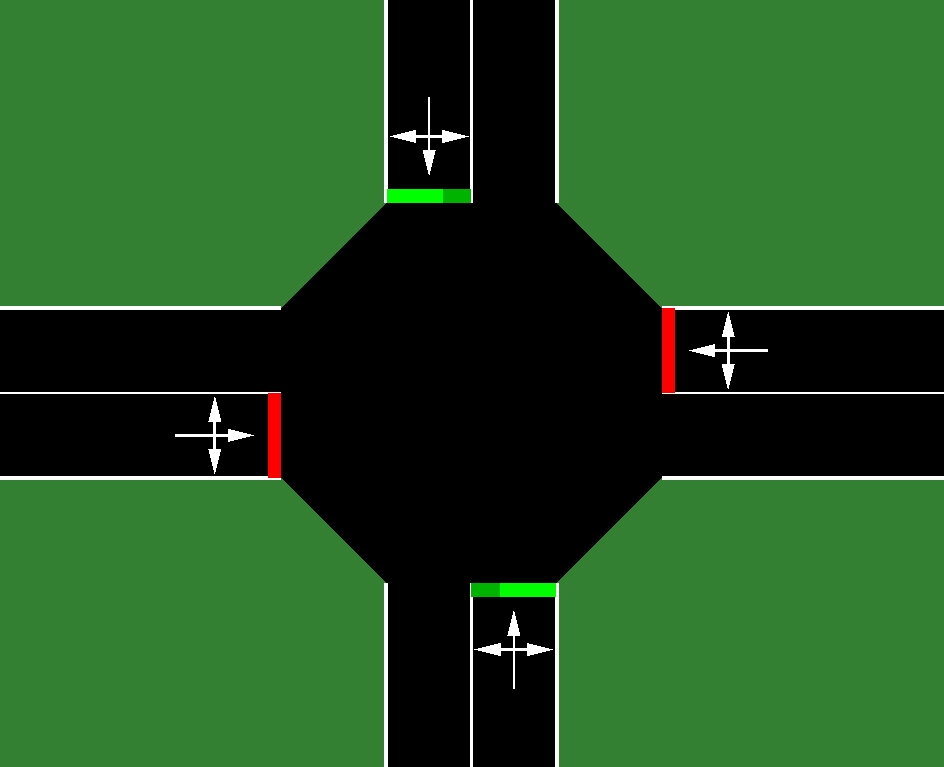
\includegraphics[width=8cm]{testcase_1.jpg}
     \caption{The used map for tests.}
     \label{fig:my_label}
 \end{figure} 


As it can be seen, there are 4 lights in the test scene. The vehicles will come from all sides of the road. The roads adjacent to each other are the same in all of the tests which uses this map.

Default red light duration is 2 minutes. Default green light duration is 30 seconds. We accept that these values are the standard traffic light values. We need to get better results in each cases in order to prove that our system is better.

For these tests we considered that the vehicles might turn right after the green light has been lighted up for them. The chance to turn right varies between 20-80\%.\cite{b1} Also, we considered that there are 3 types of vehicles in the traffic. 
These are:
\begin{itemize}
	\item Cars
	\item Buses
	\item Motorcycles
\end{itemize} 
Cars' speed varies between 50-60km/h and a constant length of 4.5m.\cite{b3} Buses' speed varies between 30-50km/h and a constant length of 14m\cite{b2}. Motorcycles' speed varies between 80-90km/h and a constant length of 2.5m.\cite{b4} By the way, these vehicles' speeds gets limited at road speed limits, so, there will be no rule breaking states in these tests.

\par Another constraint we must consider is that, the frequency of vehicle types in the traffic simulation. In our simulation, chance to create a bus is 9,2\%.\cite{b5} Chance to create a motorcycle is 7.7\%\cite{b5} and the others are cars. 
    
As you can have already noticed, there are too many random variables in these tests and this causes unreliability in the results. Because, if most of the test cases gets generated in the favor of the tests for proposed system(or vice versa), we can't say that our proposed system is better than default system or vice versa. In order to solve this problem we used the same seed value for randomization of test cases for each case. So, all of the test scenarios are the same for each test for systems. In the first test case, same cars will be generated at the same time with same amount of right turning cars in the same order. We use this test case for both of the proposed system tests and default system tests.
In the following graphs, the results are shown based on the average of multiple test results.
\subsection{Difference between vehicle amounts}

    \begin{table}[h!]
        \centering
    	\begin{tabular}{||p{0.5cm} p{2cm} p{2cm} p{1cm}||} 
    		\hline
    		\textbf{Case No.} & \textbf{Car Amount In Vertical} & \textbf{Car Amount In Horizontal} & \textbf{Time(s)} \\ [0.5ex] 
    		\hline\hline
    		1        & 30                     & 250                      & 880.71  \\ 
    		\hline
    		2        & 30                     & 300                      & 1032,7  \\
    		\hline
    		3        & 30                     & 350                      & 1175,95 \\
    		\hline
    		4        & 30                     & 400                      & 1338,2  \\
    		\hline
    		5        & 30                     & 450                      & 1462    \\
    		\hline
    	\end{tabular}
    	\newline
    	\caption{The results for default system}
    	\label{fig:my_label}
    \end{table}

The figure above represents the standard traffic light's values. The first column represents the amount of cars in the vertical road in our map. The second column represents the amount of cars in the horizontal road in our map. The third column represents the simulation's duration in seconds.
\begin{table}[h!]
	\centering
	\begin{tabular}{||p{0.5cm} p{2cm} p{2cm} p{1cm}||} 
		\hline
		\textbf{Case No.} & \textbf{Car Amount In Vertical} & \textbf{Car Amount In Horizontal} & \textbf{Time(s)} \\ [0.5ex] 
		\hline\hline
		1        & 30                     & 250                      & 865.5   \\ 
		\hline
		2        & 30                     & 300                      & 1016,1  \\
		\hline
		3        & 30                     & 350                      & 1158,25 \\
		\hline
		4        & 30                     & 400                      & 1322,5  \\
		\hline
		5        & 30                     & 450                      & 1459,75 \\
		\hline
		
	\end{tabular}
	\newline
    \caption{The results for proposed system}
    \label{fig:my_label}
\end{table}
\newline
\par The figure above represents the proposed traffic light's values. The first column represents the amount of cars in the vertical road in our map. The second column represents the amount of cars in the horizontal road in our map. The third column represents the simulation's duration in seconds.

As it can be seen from the above two tables, proposed system is much more efficient if there are uneven load of traffics in each lane. The reason behind this is simple. Let's say, there are 60 vehicles in the vertical road at the start and 30 vehicles in the horizontal one. In standard system every lane gets the same time to pass the lights. So, in the end the road with the highest amount of cars will stay congested even though other road is empty. So, the cars are losing too much time in the red light.

In our system. RSU detects how many cars each road has, then AI calculates the optimum light durations for each light. So, the road which has the highest amount of vehicles, gets more green light.
\newline

\par The duration of the lights are listed below:
\newline

\begin{table}[h!]
	\centering\textbf{Case 1:}
	\centering
	\begin{tabular}{||c c c||} 
		\hline
		\textbf{Cars} & \textbf{Red(m)} & \textbf{Green(m)} \\ [0.5ex] 
		\hline\hline
		30   & 2.21   & 0.29     \\ 
		\hline
		250  & 0.29   & 2.21     \\
		\hline
	\end{tabular}
\end{table}


\begin{table}[h!]
	\centering\textbf{Case 2:}
	\centering
	\begin{tabular}{||c c c||} 
		\hline
		\textbf{Cars} & \textbf{Red(m)} & \textbf{Green(m)} \\ [0.5ex] 
		\hline\hline
		30   & 2.25   & 0.25     \\ 
		\hline
		300  & 0.25   & 2.25     \\
		\hline
		
	\end{tabular}
\end{table}


\begin{table}[h!]
	\centering\textbf{Case 3:}
	\centering
	\begin{tabular}{||c c c||} 
		\hline
		\textbf{Cars} & \textbf{Red(m)} & \textbf{Green(m)} \\ [0.5ex] 
		\hline\hline
		30   & 2.2    & 0.3      \\ 
		\hline
		350  & 0.3    & 2.2      \\
		\hline
		
	\end{tabular}
\end{table}

% \iffalse \textbf{ADD REFERENCE \fi

\begin{table}[h!]
	\centering\textbf{Case 4:}
	\centering
	\begin{tabular}{||c c c||} 
		\hline
		\textbf{Cars} & \textbf{Red(m)} & \textbf{Green(m)} \\ [0.5ex] 
		\hline\hline
		30   & 2.3    & 0.2      \\ 
		\hline
		400  & 0.2    & 2.3      \\
		\hline
		
	\end{tabular}
\end{table}


\begin{table}[h!]
	\centering\textbf{Case 5:}
	\centering
	\begin{tabular}{||c c c||} 
		\hline
		\textbf{Cars} & \textbf{Red(m)} & \textbf{Green(m)} \\ [0.5ex] 
		\hline\hline
		30   & 2.4    & 0.1      \\ 
		\hline
		450  & 0.1    & 2.4      \\
		\hline
		
	\end{tabular}
\end{table}


 \begin{figure}[h!]
     \centering
     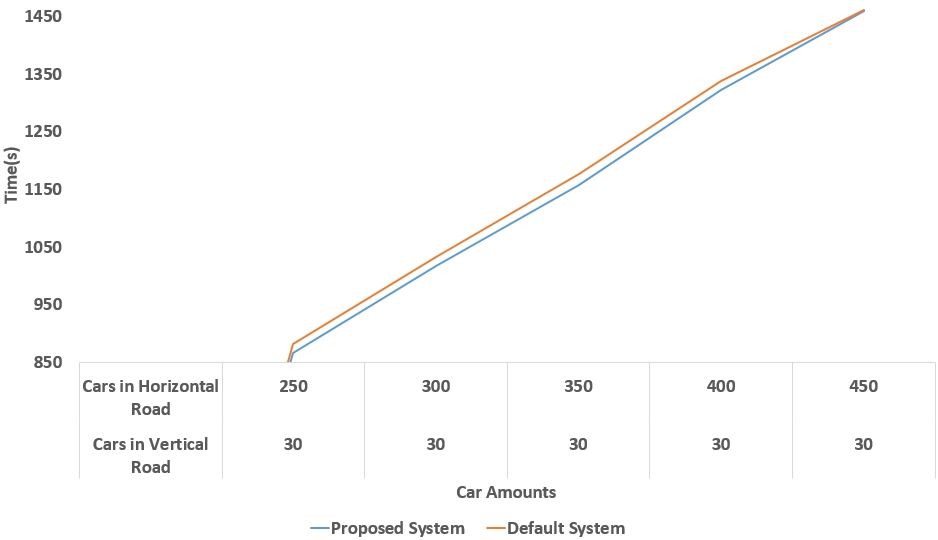
\includegraphics[width=9cm]{vehDif.jpg}
     
     \caption{Results for vehicle amount tests.}
     \label{fig:my_label}
     
 \end{figure} 



\subsection{Difference between road types}
\par For this test we have prepared 3 test areas. Those areas are a Major road(5 lanes road) vs. Street road(1 lane road), Minor road(4 lanes) vs. Street road(1 lane) and Primary road(3 lanes) vs Street road(1 lane road). 


 \begin{figure}[h!]
     \centering
     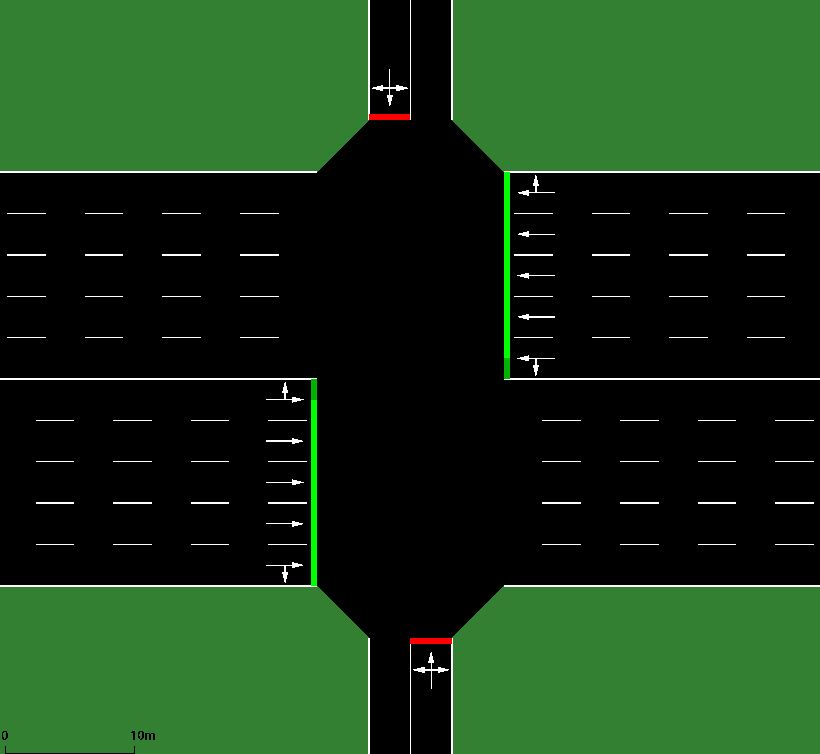
\includegraphics[width=7.5cm]{MajorvsStreet.JPG}
     \caption{Major road vs. Street road}
     \label{fig:my_label}
 \end{figure} 

 \begin{figure}[h!]
     \centering
     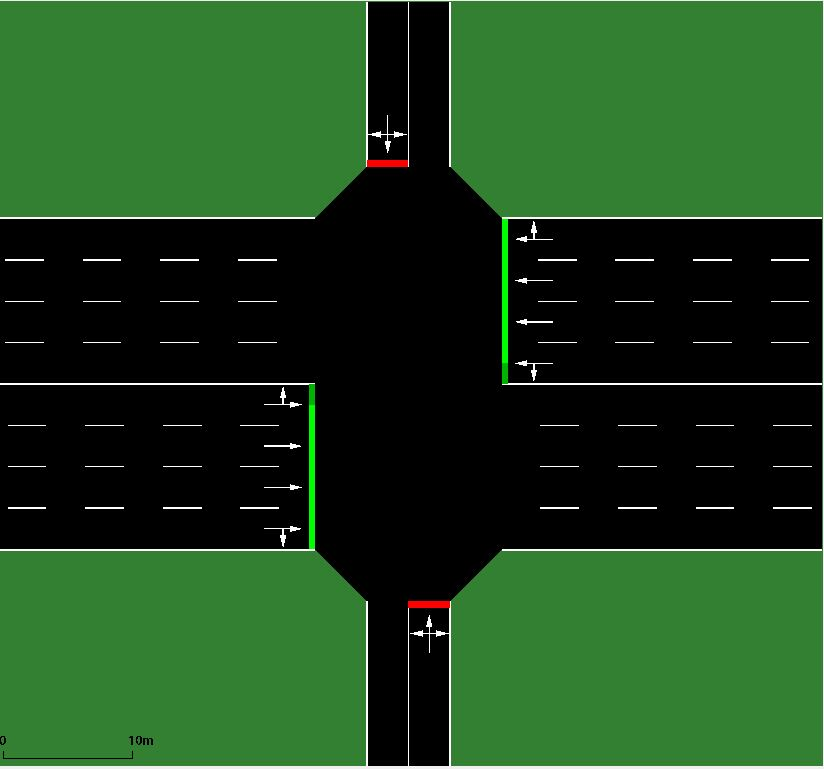
\includegraphics[width=7.5cm]{MinorvsStreet.JPG}
     \caption{Minor road vs. Street road}
     \label{fig:my_label}
 \end{figure} 
 
 \begin{figure}[h!]
     \centering
     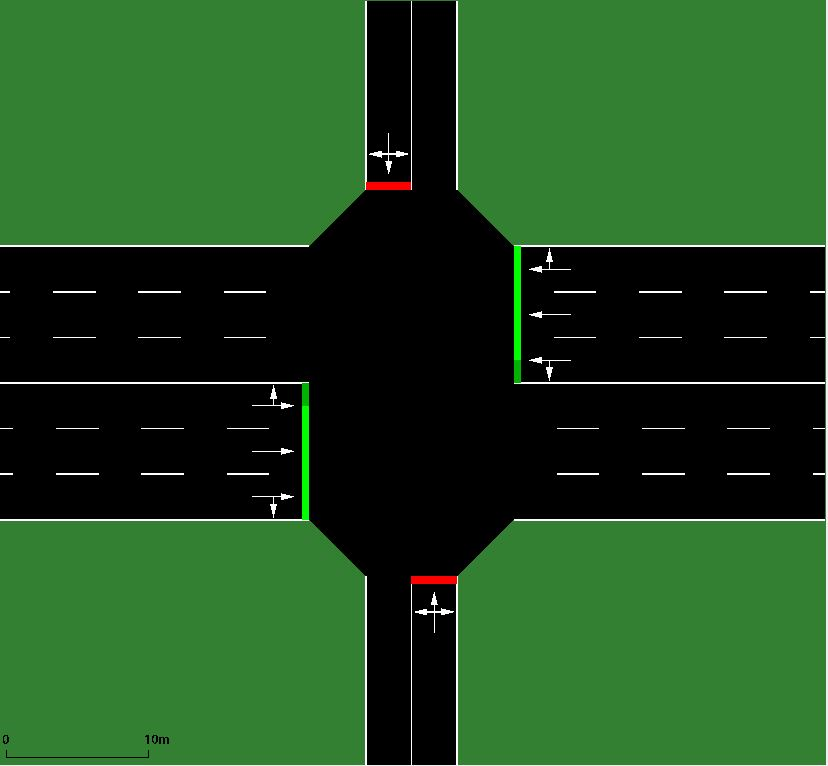
\includegraphics[width=7.5cm]{PrimaryvsStreet.JPG}
     \caption{Primary road vs. Street road}
     \label{fig:my_label}
 \end{figure} 


\par The car types and the seed amounts are the same as the previous test. For these tests the amount of vehicles in each lane is constant, which is 100. TABLE III represents the default traffic light's values.

\begin{table}[h!]
	\centering
	\begin{tabular}{||p{0.5cm} p{2cm} p{2cm} p{1cm}||} 
		\hline
		\textbf{Case No.} & \textbf{Road Type In Vertical} & \textbf{Road Type In Horizontal} & \textbf{Time(s)} \\ [0.5ex] 
		\hline\hline
		1        & Street                     & Major                      & 1350.7  \\ 
		\hline
		2        & Street                     & Minor                      & 1142.5  \\
		\hline
		3        & Street                     & Primary                      & 1142.3 \\
		\hline
	\end{tabular}
	\newline
    \caption{The results for default system}
    \label{fig:my_label}
\end{table}
	The first column shows the number of the cases. Second Column shows the road type in vertical road. Third column show the road type in the horizontal road. The fourth column show how much time needed to finish the simulation in seconds.    
    In this test, the best scenario for default system is considered. For example, in the first case the it took 1350.7 seconds in the best combination of light state sequence. So, we compare out proposed system with the best possible case for default system.
   \par TABLE IV represents the proposed traffic light's values.
    \begin{table}[h!]
	\centering
	\begin{tabular}{||p{0.5cm} p{2cm} p{2cm} p{1cm}||} 
		\hline
		\textbf{Case No.} & \textbf{Road Type In Vertical} & \textbf{Road Type In Horizontal} & \textbf{Time(s)} \\ [0.1ex] 
		\hline\hline
		1        & Street                     & Major                      & 673.1  \\ 
		\hline
		2        & Street                     & Minor                      & 800.9  \\
		\hline
		3        & Street                     & Primary                      & 815.85 \\
		\hline
	\end{tabular}
    	\newline
    	\caption{The results for proposed system}
    	\label{fig:my_label}	
\end{table}
	The first column shows the number of the cases. Second Column shows the road type in vertical road. Third column show the road type in the horizontal road. The fourth column show how much time needed to finish the simulation in seconds.
    As it can be seen that, our proposed system is much more effective than the previous test. This shows that our implementation is much more efficient at calculating lights for different road types. The duration for proposed system's calculated lights are listed below:
    
    \begin{table}[h!]
	\centering\textbf{Case 1:}
	\centering
	\begin{tabular}{||c c c||} 
		\hline
		\textbf{Road Type} & \textbf{Red(m)} & \textbf{Green(m)} \\ [0.5ex] 
		\hline\hline
		Street   & 1   & 1.5     \\ 
		\hline
		Major  & 1.5   & 1     \\
		\hline
		
	\end{tabular}
\end{table}

        \begin{table}[h!]
	\centering\textbf{Case 2:}
	\centering
	\begin{tabular}{||c c c||} 
		\hline
		\textbf{Road Type} & \textbf{Red(m)} & \textbf{Green(m)} \\ [0.5ex] 
		\hline\hline
		Street   & 0.8   & 1.7     \\ 
		\hline
		Minor  & 1 .7  & 0.8     \\
		\hline
		
	\end{tabular}
\end{table}
    
\begin{table}[h!]
	\centering\textbf{Case 3:}
	\centering
	\begin{tabular}{||c c c||} 
		\hline
		\textbf{Road Type} & \textbf{Red(m)} & \textbf{Green(m)} \\ [0.5ex] 
		\hline\hline
		Street   & 0.8   & 1.7     \\ 
		\hline
		Primary  & 1 .7  & 0.8     \\
		\hline
		
	\end{tabular}
\end{table}

 \begin{figure}[h!]
     \centering
     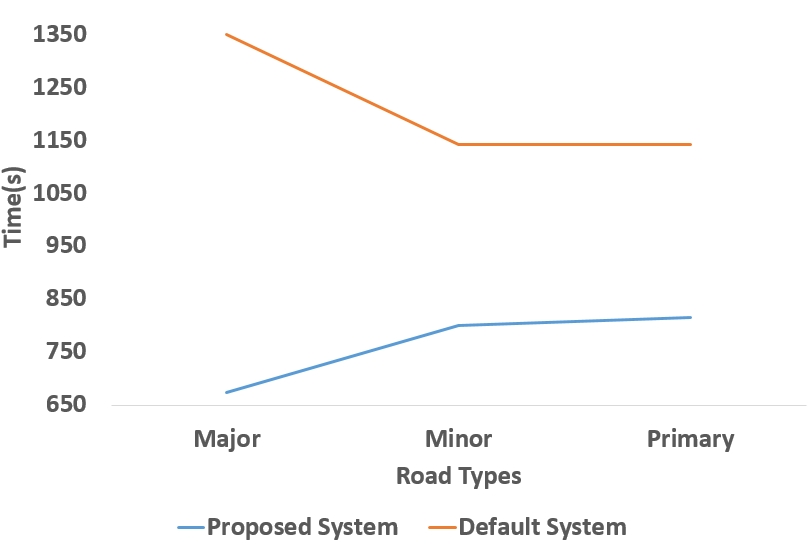
\includegraphics[width=8.5cm]{roadTypes.jpg}
     \caption{Results for road types}
     \label{fig:my_label}
 \end{figure}   
 
\section{Future Works}
    \par In our proposed system, we have discussed about an AI which we have implemented in a short time. So, it creates opportunities for improvements.
    \par One of the improvements might be considering deep learning into our system. In our system there is no pre-trained AI. So, there is still room for improvement. With deep learning, AI can predict best light duration better than using some constraints pre-defined by a user. These constraints are just some numbers which would be used for weights in a neural network.
    \par Another improvement for the AI might be, including more variables into to consideration. In section VI, we have shown what those variables are. In addition, pedestrians, accidents...etc. might also be considered.
    \par Aside from AI, there is room for improvements for RSU. For example, in our proposed system, there is no vehicle-to-vehicle communication. There is only vehicto-to-RSU communication. So, vehicle-to-vehicle communication might also be considered while implementing the system in real life. So, the problem occured by obstacles for RSU-to-AI will be minified.
    
\section{Conclusion}
    \par In this paper we have compared an AI oriented smart traffic light system with a traditional system to observe and provide a new solution on modern congestion problems.
    \par Proposed system tested in a traffic simulation environment. In those, simulations we have tested both of the traffic light aligning methods in the same traffic flow. So, we have managed to validate our tests' reliability. Also, added more than one type of vehicle and ability to turning right when the light hit green is added to further increase the reliability and realism of our tests. According to those tests we have validated that our proposed system is much more better than the default system as can be observed at performance evaluation section.



\begin{thebibliography}{00}
\bibitem{a1} Phil Goodwin (2004) The Economic Costs of Road Traffic Congestion 
\bibitem{b1} http://www.mikeontraffic.com/study-results-right-turn-red-percentages/
\bibitem{b2} https://itstillruns.com/standard-size-city-bus-7440823.html
\bibitem{b3} https://mechanicbase.com/cars/average-car-length
\bibitem{b4} http://www.motorcycleguidelines.org.uk/the-guidelines/6-0-motorcycle-parking/6-5-motorcycle-parking-resources/
\bibitem{b5} https://ec.europa.eu/eurostat/statistics-explained/pdfscache/14273.pdf
\bibitem{b6} Andre Maia Pereira, "Traffic signal control for connected and non-connected vehicles", Smart City Symposium Prague (SCSP) 2018, pp. 1-6, 2018.
\bibitem{b7} Mishra,Sumit And Bhattacharya, Devanjan And Gupta, Ankit. (2018). Congestion Adaptive Traffic Light Control and Notification Architecture Using Google Maps APIs
\bibitem{b8} V. Gupta, R. Kumar, K. S. Reddy and B. K. Panigrahi, "Intelligent traffic light control for congestion management for smart city development," 2017 IEEE Region 10 Symposium (TENSYMP), Cochin, 2017, pp. 1-5.


\end{thebibliography}
\end{document}